\subsection{Seleccionar una técnica de modelado}

Para este trabajo decidimos utilizar dos técnicas de modelado, J48 Decision Tree
y Multilayer Perceptron. El motivo por el que elegimos estas técnicas es porque
son algoritmos supervisados, lo cual es adecuado para el problema que intentamos
resolver, y porque estos algoritmos, al funcionar sobre principios diferentes,
reaccionan de distinta forma ante distintos tipos de datos de entrada,
permitiéndonos de esta forma compararlos, y elegir el más apropiado.
Se Aplicará cada una de estas técnicas, variando sus parámetros
para obtener mejores resultados.
La clase para estos algoritmos será el atributo \code{is\_successfull}, el cual
surgirá de aplicar una función de threshold a la cantidad de views de cada
video. Para evitar que el algoritmo tenga información relacionada directamente
con la clase, quitaremos el atributo \code{views} del set de datos para aplicar
los algoritmos.

    \subsubsection{Técnica de modelado}
      \textbf{J48 Decision Tree:} Se utilizará el algoritmo supervisado J48, el cual
      consiste en un árbol de decisión utilizado para la clasificación del set
      de datos.\\
      \textbf{Multilayer Perceptron:} Se utilizará el algoritmo supervisado
      Multilayer Perceptron, el cual consiste en una Red Neuronal del tipo
      backtracking, utilizado para la clasificación del set de datos.

    \subsubsection{Supuestos de modelado}
        Todos los datos usados para el modelado son numéricos, booleanos

\subsection{Generar el diseño de las pruebas}
    \subsubsection{Diseño de las pruebas}

      Para ambas técnicas de modelado se eligió utilizar un 70 \% del dataset
      como set de entrenamiento y un 30 \% del dataset comos set de prueba,
      elegido al azar (se mezcla al azar todo el set de pruebas y se elige el
      70 \% de los registros que se encuentran primero). Se escogió de esta forma
      para darle suficientes datos a la red neuronal. En total quedan 1906
      registros para prueba y 4445 registros para entrenamiento.


\subsection{Construir el modelo}
    \subsubsection{Configuración de parámetros}

      \paragraph{Arbol J48}
          Para el caso del árbol J48 debemos ajustar los parámetros de nivel de
          confianza y cantidad mínima de elementos por hoja.\\\\
          \textbf{Nivel de Confianza\\}
          Un nivel de confianza demasiado alto provocará que el algoritmo no
          desestime ninguna regla lo cual llevará a un posible overfit.\\\\
          \textbf{Cantidad mínima de Elementos por hoja\\}
          Lo mismo puede ocurrir en caso de usar un valor demasiado bajo de
          cantidad minima de elementos por hoja.\\
          Luego de Experimentar con distintos valores para cada caso, llegamos a
          los siguientes valores que nos dan los mejores resultados:

          \subparagraph{Parámetros para el arbol 1}

            \begin{tabular}{||c | c||}
                \hline
                \textbf{Parametro} & \textbf{valor} \\ [0.5ex]
                \hline\hline
                Confidence Level & 0.1 \\
                \hline
                Minium elements per Leaf & 3 \\
                \hline
            \end{tabular}

          \subparagraph{Parámetros para el arbol 2}

            \begin{tabular}{||c | c||}
                \hline
                \textbf{Parametro} & \textbf{valor} \\ [0.5ex]
                \hline\hline
                Confidence Level & 0.3 \\
                \hline
                Minium elements per Leaf & 20 \\
                \hline
            \end{tabular}

         \hfill \break
         \hfill \break
          Luego de varios test, notamos que el valor de Minium elements per leaf
          que mejor resultado en términos de precisión era 60, pero el árbol
          quedaba demasiado grande como para comprenderlo fácilmente. Decidimos
          subirlo a 80 para obtener un árbol razonable, perdiendo una cantidad
          despreciable de precisión. Subirlo a mas de 80 ya podaba mucho el
          árbol y generaba pérdidas de precisión importantes.\\
          De la misma forma elegimos un Confidence level de 0.01. Disminuirlo
          mas generaba una pérdida de precisión, aumentarlo nos resultaba en un
          arbol mucho mas grande.

      \paragraph{Multilayer Perceptron}
          Para el caso del Multilayer Perceptron debemos ajustar la cantidad
          hidden layers, el learning rate, el momentum, el training time y el
          decay.\\\\
          \textbf{Hidden Layers\\}
          Si se colocan demasiadas hidden layers se incrementa mucho el tiempo
          de procesamiento, y ademas se corre el riesgo de overfiting. Si se
          colocan muy pocas puede que no sean suficientes para aproximar
          correctamente la función del problema.\\\\
          \textbf{Learning Rate\\}
          El learning rate y el momentum afectan la velocidad a la que intenta
          converger el algoritmo. Un learning rate o momentum demasiado elevador
          provocaran que el algoritmo no logre encontrar un mínimo local. Un
          learning rate o momentum demasiado pequeños provocan que el algoritmo
          no logre encontrar un mínimo global.\\\\
          \textbf{Training Time\\}
          Es la cantidad de pasadas de los datos a través de la red. Aumentarlo
          debería mejorar los resultados, sin embargo incrementa el tiempo de
          procesamiento y puede provocar overfiting.\\\\
          \textbf{Decay\\}
          Si está activado El algoritmo Cambia dinámicamente el learning rate
          según los resultados anteriores. Sirve para evitar que el algoritmo
          se pase por alto los mínimos, pero aumenta el tiempo de
          procesamiento.\\\\
          Luego de Experimentar con distintos valores para cada caso, llegamos a
          los siguientes valores que nos dan los mejores resultados:
          \subparagraph{Parámetros}
                \begin{tabular}{||c | c||}
                    \hline
                    \textbf{Parametro} & \textbf{valor} \\ [0.5ex]
                    \hline\hline
                    Hidden Layers & 30 \\
                    \hline
                    Momentum & 0.2 \\
                    \hline
                    Learing Rate & 0.3 \\
                    \hline
                    Training Time & 500 \\
                    \hline
                    Decay & Desactivado \\
                    \hline
                \end{tabular}
    \newpage
    \subsubsection{Modelos}

        \def\RUN{1}
        \def\title{Resultados de la corrida 1 del arbol de decisión J48}
        \def\algorithm{weka}
        \def\numberOfRules{17}
        \def\hasRules{1}
        \paragraph{\title}
    \subparagraph{Matriz de confusion}

        \begin{figure}[ht]
            \begin{adjustbox}{addcode={
                \begin{minipage}{\width}}{
                \end{minipage}},rotate=360,center}
                \includegraphics[scale=.6]{\algorithm_\RUN_confusion_matrix.png}
            \end{adjustbox}
        \end{figure}
        \FloatBarrier

    \subparagraph{Resultados de la clasificación}

        \begin{figure}[ht]
            \begin{adjustbox}{addcode={
                \begin{minipage}{\width}}{
                \end{minipage}},rotate=360,center}
                \includegraphics[scale=.6]{\algorithm_\RUN_clasification_results.png}
            \end{adjustbox}
        \end{figure}
        \FloatBarrier

    \if\hasRules1
        \newpage
        \subparagraph{Reglas}
            \foreach \x in {0, ..., \numberOfRules} {
                \begin{itemize}
                    \item \textbf{Regla \x}:
                    \begin{figure}[ht]
                        \begin{adjustbox}{addcode={
                            \begin{minipage}{\width}}{
                              %\caption{Regla \x}
                            \end{minipage}},rotate=360,center}
                            \includegraphics[scale=.6]{weka_\RUN_rule\x.png}
                            \includegraphics[scale=.6]{weka_\RUN_rule\x_calculations.png}
                        \end{adjustbox}
                    \end{figure}
                    \FloatBarrier
              \end{itemize}
            }

        \newpage
        \subparagraph{Arbol}

            \begin{figure}[ht]
                \begin{adjustbox}{addcode={
                    \begin{minipage}{\width}}{
                        \caption{Arbol de desicion}
                    \end{minipage}},rotate=360,center}
                    \includegraphics[scale=.4]{tree_\RUN.png}
                \end{adjustbox}
            \end{figure}
            \FloatBarrier
        \newpage
    \fi
        \newpage

        \def\RUN{2}
        \def\title{Resultados de la corrida 2 del arbol de decisión J48}
        \def\algorithm{weka}
        \def\numberOfRules{20}
        \def\hasRules{1}
        \paragraph{\title}
    \subparagraph{Matriz de confusion}

        \begin{figure}[ht]
            \begin{adjustbox}{addcode={
                \begin{minipage}{\width}}{
                \end{minipage}},rotate=360,center}
                \includegraphics[scale=.6]{\algorithm_\RUN_confusion_matrix.png}
            \end{adjustbox}
        \end{figure}
        \FloatBarrier

    \subparagraph{Resultados de la clasificación}

        \begin{figure}[ht]
            \begin{adjustbox}{addcode={
                \begin{minipage}{\width}}{
                \end{minipage}},rotate=360,center}
                \includegraphics[scale=.6]{\algorithm_\RUN_clasification_results.png}
            \end{adjustbox}
        \end{figure}
        \FloatBarrier

    \if\hasRules1
        \newpage
        \subparagraph{Reglas}
            \foreach \x in {0, ..., \numberOfRules} {
                \begin{itemize}
                    \item \textbf{Regla \x}:
                    \begin{figure}[ht]
                        \begin{adjustbox}{addcode={
                            \begin{minipage}{\width}}{
                              %\caption{Regla \x}
                            \end{minipage}},rotate=360,center}
                            \includegraphics[scale=.6]{weka_\RUN_rule\x.png}
                            \includegraphics[scale=.6]{weka_\RUN_rule\x_calculations.png}
                        \end{adjustbox}
                    \end{figure}
                    \FloatBarrier
              \end{itemize}
            }

        \newpage
        \subparagraph{Arbol}

            \begin{figure}[ht]
                \begin{adjustbox}{addcode={
                    \begin{minipage}{\width}}{
                        \caption{Arbol de desicion}
                    \end{minipage}},rotate=360,center}
                    \includegraphics[scale=.4]{tree_\RUN.png}
                \end{adjustbox}
            \end{figure}
            \FloatBarrier
        \newpage
    \fi
        \newpage

        \def\RUN{1}
        \def\title{Resultados de la corrida de Perceptron}
        \def\algorithm{perceptron}
        \def\numberOfRules{20}
        \def\hasRules{0}
        \paragraph{\title}
    \subparagraph{Matriz de confusion}

        \begin{figure}[ht]
            \begin{adjustbox}{addcode={
                \begin{minipage}{\width}}{
                \end{minipage}},rotate=360,center}
                \includegraphics[scale=.6]{\algorithm_\RUN_confusion_matrix.png}
            \end{adjustbox}
        \end{figure}
        \FloatBarrier

    \subparagraph{Resultados de la clasificación}

        \begin{figure}[ht]
            \begin{adjustbox}{addcode={
                \begin{minipage}{\width}}{
                \end{minipage}},rotate=360,center}
                \includegraphics[scale=.6]{\algorithm_\RUN_clasification_results.png}
            \end{adjustbox}
        \end{figure}
        \FloatBarrier

    \if\hasRules1
        \newpage
        \subparagraph{Reglas}
            \foreach \x in {0, ..., \numberOfRules} {
                \begin{itemize}
                    \item \textbf{Regla \x}:
                    \begin{figure}[ht]
                        \begin{adjustbox}{addcode={
                            \begin{minipage}{\width}}{
                              %\caption{Regla \x}
                            \end{minipage}},rotate=360,center}
                            \includegraphics[scale=.6]{weka_\RUN_rule\x.png}
                            \includegraphics[scale=.6]{weka_\RUN_rule\x_calculations.png}
                        \end{adjustbox}
                    \end{figure}
                    \FloatBarrier
              \end{itemize}
            }

        \newpage
        \subparagraph{Arbol}

            \begin{figure}[ht]
                \begin{adjustbox}{addcode={
                    \begin{minipage}{\width}}{
                        \caption{Arbol de desicion}
                    \end{minipage}},rotate=360,center}
                    \includegraphics[scale=.4]{tree_\RUN.png}
                \end{adjustbox}
            \end{figure}
            \FloatBarrier
        \newpage
    \fi

    \subsubsection{Análisis de predicciones de clasificación}

        A continuación presentamos algunos gráficos que muestran la tendencia
        del algoritmo a clasificar correcta o incorrectamente los eventos, según
        sus atributos

        \begin{figure}[ht]
            \begin{adjustbox}{addcode={
                \begin{minipage}{\width}}{
                    \caption{Clasif. Errors vs tag length}
                \end{minipage}},rotate=360,center}
                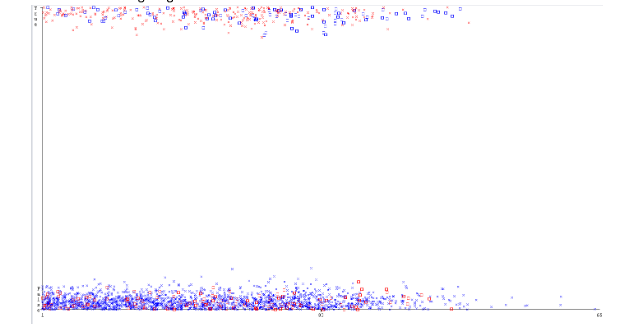
\includegraphics[scale=.6]{clasif_error_tags_length.png}
            \end{adjustbox}
        \end{figure}
        \FloatBarrier

        Podemos observar en este gráfico que los videos con muchos tags tienen
        menos chance de ser exitosos, algo que ya habíamos visto en la etapa de
        conocimiento del negocio, notando además que para los videos que tienen
        muchos tags, aquellos clasificados como exitosos son en su mayoría
        falsos positivos, esta información puede ser útil para futuros análisis.

        \begin{figure}[ht]
            \begin{adjustbox}{addcode={
                \begin{minipage}{\width}}{
                    \caption{Clasif. errors vs title length}
                \end{minipage}},rotate=360,center}
                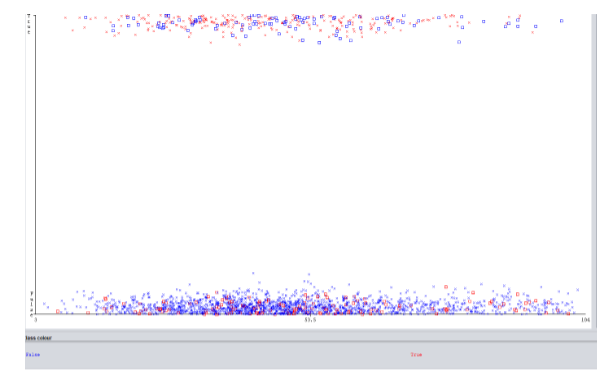
\includegraphics[scale=.6]{clasif_error_title_length.png}
            \end{adjustbox}
        \end{figure}
        \FloatBarrier

        Vemos que los videos que tienen títulos demasiado largos tienen menos
        chance de ser exitosos, tal como nos muestran las reglas, y además vemos
        que el algoritmo identifica correctamente estos casos, teniendo un alto
        porcentaje de acierto tanto en positivos como en negativos.

        \begin{figure}[ht]
            \begin{adjustbox}{addcode={
                \begin{minipage}{\width}}{
                    \caption{Clasif. errors vs category}
                \end{minipage}},rotate=360,center}
                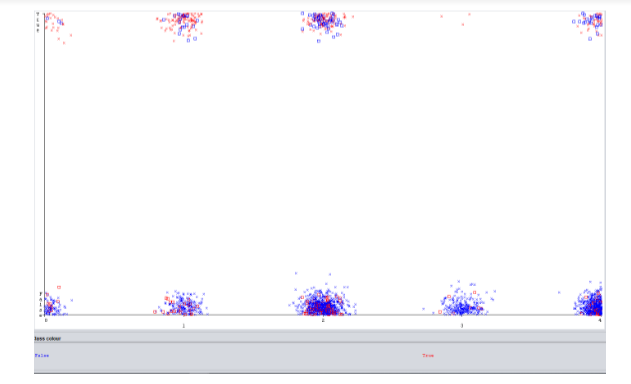
\includegraphics[scale=.6]{clasif_error_category.png}
            \end{adjustbox}
        \end{figure}
        \FloatBarrier

        En este gráfico vemos por un lado, que los grupos de categorías 3 y 4
        tienen poca cantidad de videos exitosos, a pesar que tienen mucha
        cantidad de videos, y por otro lado notamos que el algoritmo es muy
        efectivo clasificando videos pertenecientes a los grupos 0, 1 y 3, y
        no tan efectivo al clasificar los videos de grupos 2 y 4.

        \begin{figure}[ht]
            \begin{adjustbox}{addcode={
                \begin{minipage}{\width}}{
                    \caption{Clasif. errors vs like ratio}
                \end{minipage}},rotate=360,center}
                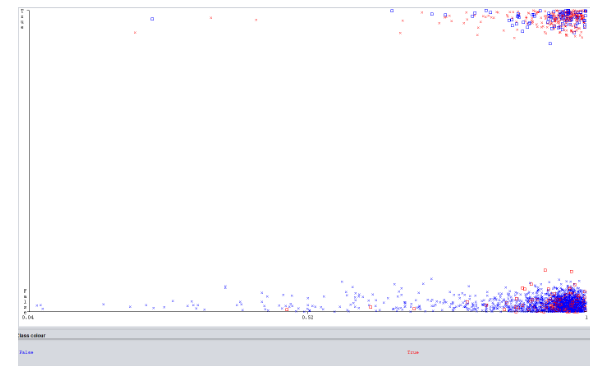
\includegraphics[scale=.6]{clasif_error_likes_ratio.png}
            \end{adjustbox}
        \end{figure}
        \FloatBarrier

        Este gráfico es interesante, vemos muy claramente que los videos que
        tienen poco like ratio tienen mucha menos chance de ser exitosos, y
        además el algoritmo los clasifica casi perfectamente, mientras que los
        videos con un like ratio mayor tienen más chance de ser exitosos, pero
        el algoritmo es menos efectivo al clasificarlos correctamente.

        \newpage

    \subsubsection{Descripción del modelo}
\subsection{Evaluar el modelo}
    \subsubsection{Evaluación del modelo}
        \paragraph{Analisis de reglas}
            \begin{itemize}
                \item \textbf{Arbol 1:}
                \begin{itemize}
                    \item \textbf{Regla 2}: Podemos apreciar que el progreso
                    del video es un factor decisivo ya que el promedio de vistas
                    por dia desde su publicacion determina el exito del video
                    \item \textbf{Regla 3}: Podemos apreciar que el hecho de que
                    la categoria es importante porque nos dice que el exito del
                    video se basa en que la gente prefiere cierto contenido
                    relacionado a peliculas, animacion, comedia, etc
                    \item \textbf{Regla 4}: Podemos ver que la cantidad de tag
                    juega un rol importante ya que juega como promotor del mismo,
                    es decir, los tags facilitan la busqueda del video ya que los
                    mismos se pueden buscar por tags, entonces estos te permiten
                    llegar a la gente.
                    \item \textbf{Regla 5}: Podemos ver que el tamaño del titulo
                    juega un rol principal ya que tener un maximo del largo del
                    mismo nos dice que la curiosidad de la gente se despierta
                    frente a titulos de cierto rango de tamaño.
                \end{itemize}
                \item \textbf{Arbol 2:}
                \begin{itemize}
                    \item  \textbf{Reglas 0 y 1:} Esta regla nos muestra que
                    cuando un video no comienza con un crecimiento elevado,
                    entonces es dificil que pueda llegar a ser un video exitoso,
                    por lo que parece ser que los videos con bajo crecimiento
                    tienen poca probabilidad de llegar a ser exitosos.

                    \item \textbf{Regla 2:} En esta regla podemos ver que los
                    videos que comienzan con buen crecimiento y son de la
                    categoria 0 tienen alta probabilidad de ser exitosos. Esto
                    es razonable ya que la categoria 0 corresponde a los videos
                    de peliculas y animacion, cuyo exito o no suele definirse
                    en cuanto son subidos.

                    \item \textbf{Regla 3:} Esta regla muestra que los videos de
                    cierta categoria tienen mas chances de ser exitoso. Ademas
                    nos presenta como requisito que tenga una cierta cantidad
                    de likes ratio, lo que nos muestra que la cantidad de likes
                    influye en la popularidad y el exito de los videos.

                    \item \textbf{Regla 5:} Esta regla puede deberse a que la
                    gente navega muy rapido buscando videos, y los titulos mas
                    cortos se pueden leer mas rapidamente. A su vez, en la
                    categoria que nos muestra de blogs y entretenimiento suelen
                    ubicarse los videos de canales exitosos, los cuales por lo
                    general tienen titulos cortos y, al tener muchos seguidores
                    el canal en si, tienen mas cantidad de views.

                    \item \textbf{Regla 10:} Esta tiene una confianza muy alta
                    y una captura razonable, pero simplemente nos muestra que
                    los videos de categoria 1 suelen ser exitosos lo cual
                    coincide con nuestro conocimiento previo ya que los videos
                    de musica son los mas populares de youtube.

                    \item \textbf{Regla 11:} Esta regla tiene una confianza y
                    captura razonables, y nos muestra que los videos de
                    entretenimiento y blogging que tienen menos de 25 tags
                    tienen mas chances de ser exitosos. Una explicacion de esto
                    podria ser por la inversa, es decir que los videos que
                    tienen demasiados tags son menos exitosos, ya que
                    probablemente son videos largos que abarcan muchos temas y
                    por lo general menos views.

                    \item \textbf{Regla 16:} Regla tiene poca captura y poco
                    soporte, pero una confianza muy alta, lo que significa que
                    identifica un nicho, y tiene sentido que son videos de una
                    categoria que no es de las mas comunes, que tienen titulos
                    muy largos, y una cantidad bajas de likes, por lo que
                    parecen ser videos polemicos, que terminan siendo exitosos
                    debido justamente a la polemica generado por estos mismos.

                    \item \textbf{Regla 20:} Esta regla muestra algo que
                    habiamos visto en el entendimiento del negocio y es que los
                    videos con titulos extremadamente largos tienen menos
                    chances de exito.

                    \item \textbf{Regla 4, 6, 8, 13 y 18:} Estas reglas tienen
                    poca confianza, por lo que no resulta muy apropiado tener
                    en cuenta sus resultados ya que pueden llevar a errores.

                    \item \textbf{Regla 7, 9, 12, 15, 17 y 19:} Estas reglas
                    tienen poca captura y soporte, por lo que no son
                    representativas de la poblacion, y tampoco parecieran
                    señalar algun nicho ya que sus confianzas no son tan altas.

                \end{itemize}
            \end{itemize}

    \subsubsection{Revisión de la configuración de parámetros}
        Para lograr una buena construcción del árbol, se limitó la cantidad de
        nodos hoja a valores peequeños como 3 y 20 ya que nos da una cantidad
        de reglas razonable y a menos cantidad nos daban reglas mas chicas y
        en mas cantidad.\\
        Se probó variar la cantidad mínima de muestras requerida para hacer
        un split, la cantidad mínima de muestras que debe haber en un nodo
        hoja, la cantidad máxima de niveles del árbol.

